
%%%%%%%%%%%%%%%%%%%%%%%%%%%%%%%%%%%%%%%%%%%%%%%%%%%%%%%%%%%%%%%%%%%%%%%%%%%%%%%%
%% 

\cleardoubleoddpage % Start results on a new odd page
\chapter{Results}
\label{sec:results}

This chapter reports the empirical findings. All procedures and metrics are defined in
Section~\ref{sec:methods}. We first examine how engagement relates to sentiment,
then present genre-wise sentiment distributions and polarization, analyze the hip-hop
anomaly, study views versus sentiment, investigate emoji usage, and finally connect
LIWC patterns with VADER sentiment.


\section{Engagement--Sentiment Correlation}
\label{subsec:results_engagement}

We analyze the relationship between expressed sentiment and audience engagement, measured
by comment \texttt{like\_count}. For each genre, we compute Spearman rank correlations 
between likes and the four VADER sentiment dimensions (\texttt{positive}, \texttt{negative},
\texttt{neutral}, and \texttt{compound}), with 95\% confidence intervals.

\subsection*{Positive Sentiment (VADER\_pos)}
Genres such as \textit{Nu Jazz}, \textit{Disco}, and \textit{Latin Rock} show positive 
correlations ($\rho \approx 0.12$), suggesting that positivity is modestly rewarded. 
By contrast, \textit{Grime} ($\rho = -0.06$), \textit{Teen Pop} ($\rho = -0.07$), and 
\textit{Video Game Music} ($\rho = -0.10$) exhibit negative associations, where positive 
comments appear to be less endorsed.

\begin{figure}[htbp]
    \centering
    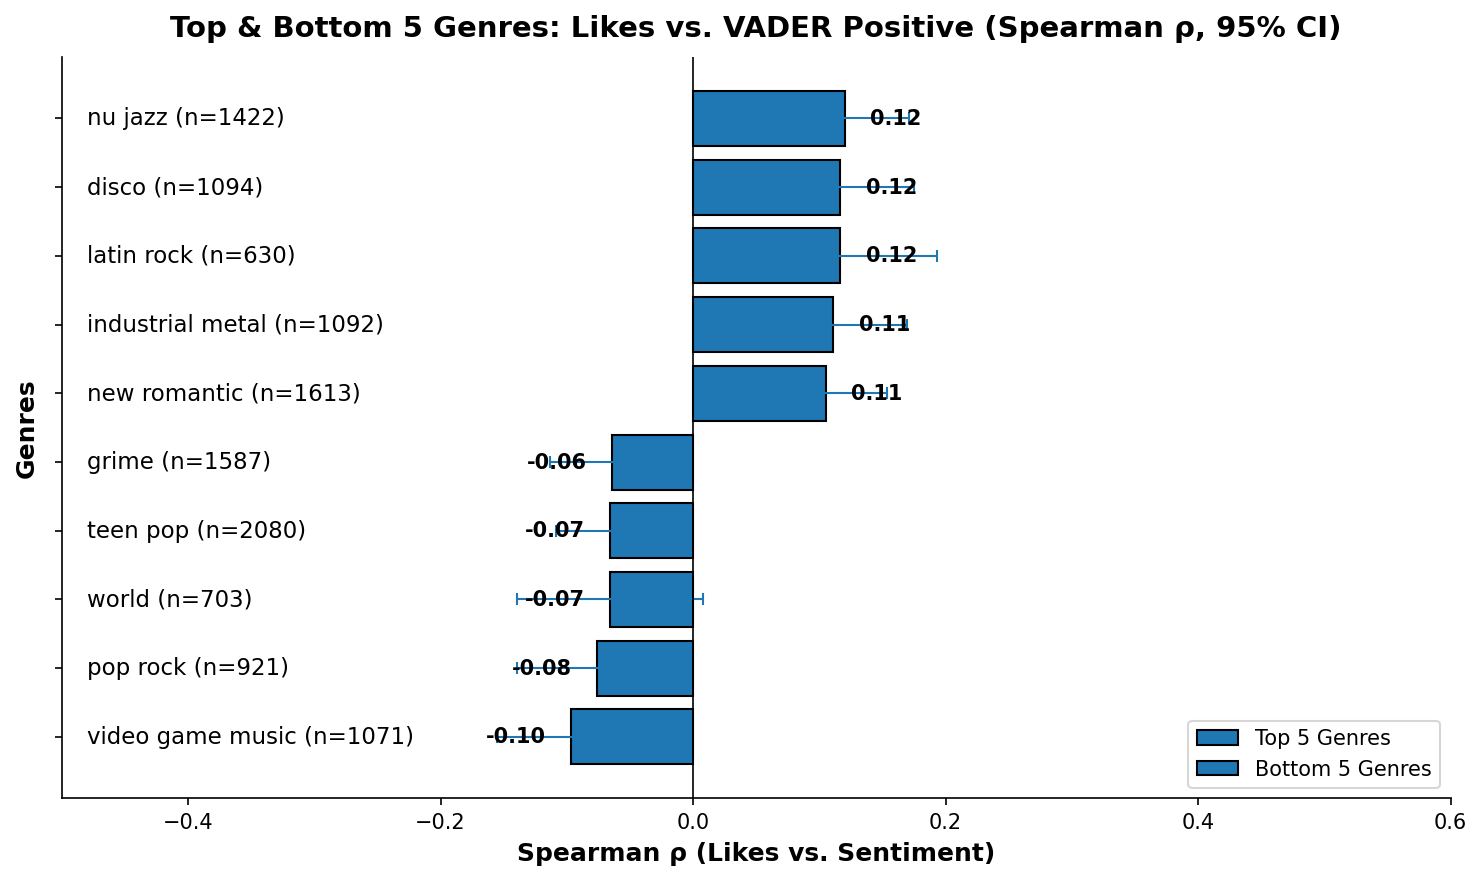
\includegraphics[width=0.85\textwidth]{images/spear_likes_pos_tb5.png}
    \caption{Top and bottom five genres by correlation between likes and VADER positive sentiment.}
    \label{fig:spear_likes_pos}
\end{figure}
\FloatBarrier

\subsection*{Negative Sentiment (VADER\_neg)}
Interestingly, \textit{Singer-Songwriter} ($\rho = 0.12$), \textit{Folk} ($\rho = 0.11$), 
and \textit{Contemporary Classical} ($\rho = 0.10$) show positive correlations, indicating 
that more negative comments can still gain approval in reflective or critical communities. 
Conversely, \textit{Country Pop}, \textit{Swing}, and \textit{Latin Rock} all show 
negative correlations around $\rho \approx -0.08$ to $-0.10$, where negativity is less validated.

\begin{figure}[htbp]
    \centering
    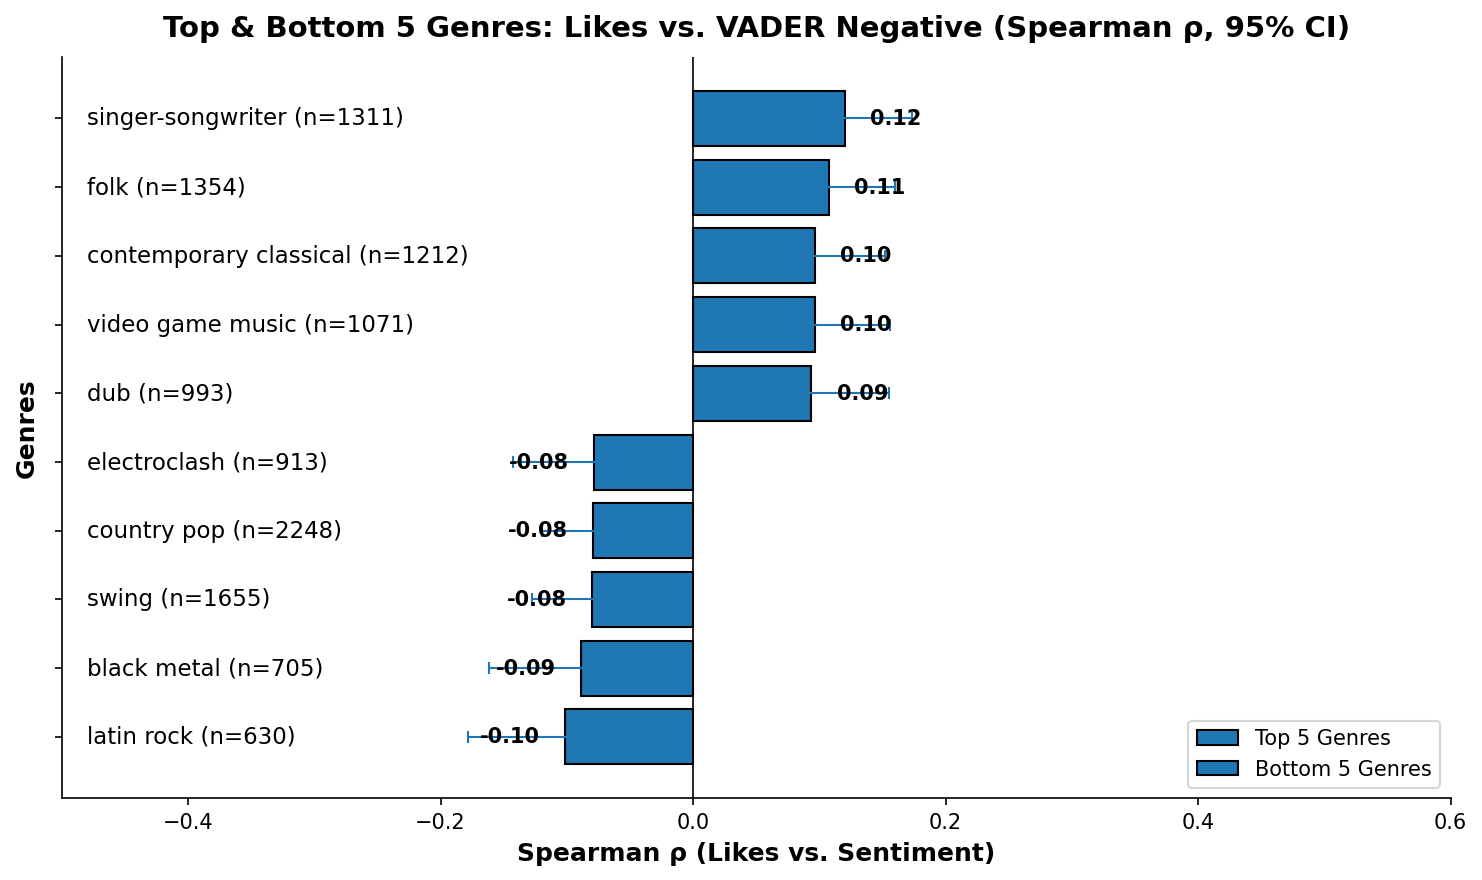
\includegraphics[width=0.85\textwidth]{images/spear_likes_neg_tb5.png}
    \caption{Top and bottom five genres by correlation between likes and VADER negative sentiment.}
    \label{fig:spear_likes_neg}
\end{figure}
\FloatBarrier

\subsection*{Neutral Sentiment (VADER\_neu)}
\textit{World} ($\rho = 0.08$), \textit{Breakbeat} ($\rho = 0.08$), and \textit{Garage Punk} 
($\rho = 0.07$) show weak positive correlations, suggesting that neutral-toned comments 
can still attract likes. By contrast, \textit{Baroque} ($\rho = -0.08$), 
\textit{Nu Jazz} ($\rho = -0.09$), and \textit{Girl Group} ($\rho = -0.09$) 
exhibit small negative correlations, where neutrality appears less rewarded.

\begin{figure}[htbp]
    \centering
    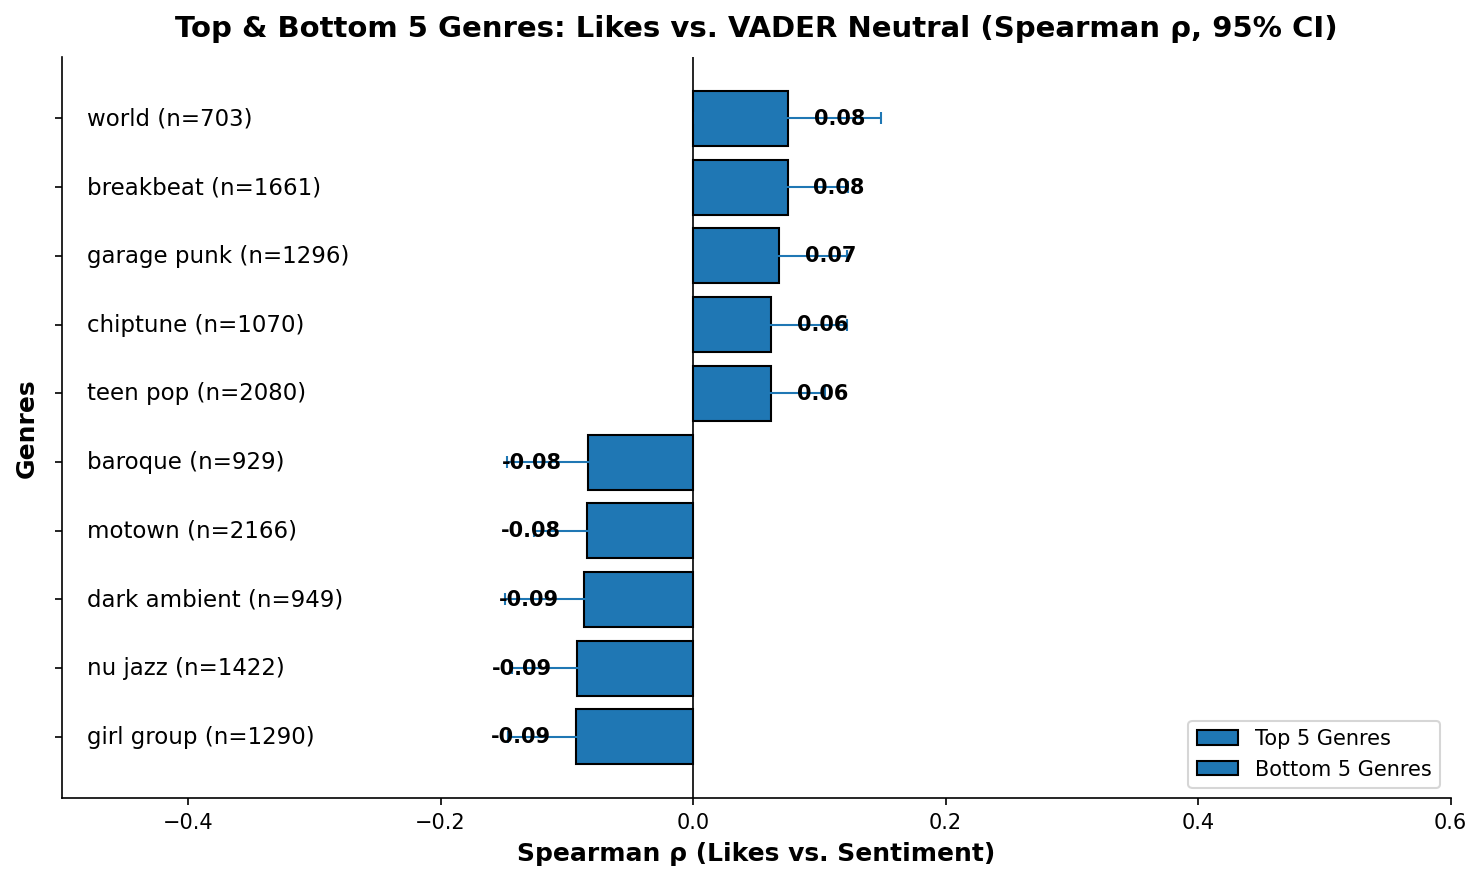
\includegraphics[width=0.85\textwidth]{images/spear_likes_neu_tb5.png}
    \caption{Top and bottom five genres by correlation between likes and VADER neutral sentiment.}
    \label{fig:spear_likes_neu}
\end{figure}
\FloatBarrier

\subsection*{Compound Sentiment (VADER\_compound)}
The overall sentiment score shows the strongest patterns. Genres such as 
\textit{Nu Jazz}, \textit{Disco}, \textit{Jangle Pop}, and \textit{Madchester} 
all show positive correlations ($\rho \approx 0.17$), while \textit{Latin Rock} 
follows closely with $\rho = 0.16$. At the other end, \textit{Grime} ($\rho = -0.03$), 
\textit{Teen Pop} ($\rho = -0.02$), and \textit{Video Game Music} ($\rho = -0.09$) 
show weak negative correlations.

\begin{figure}[htbp]
    \centering
    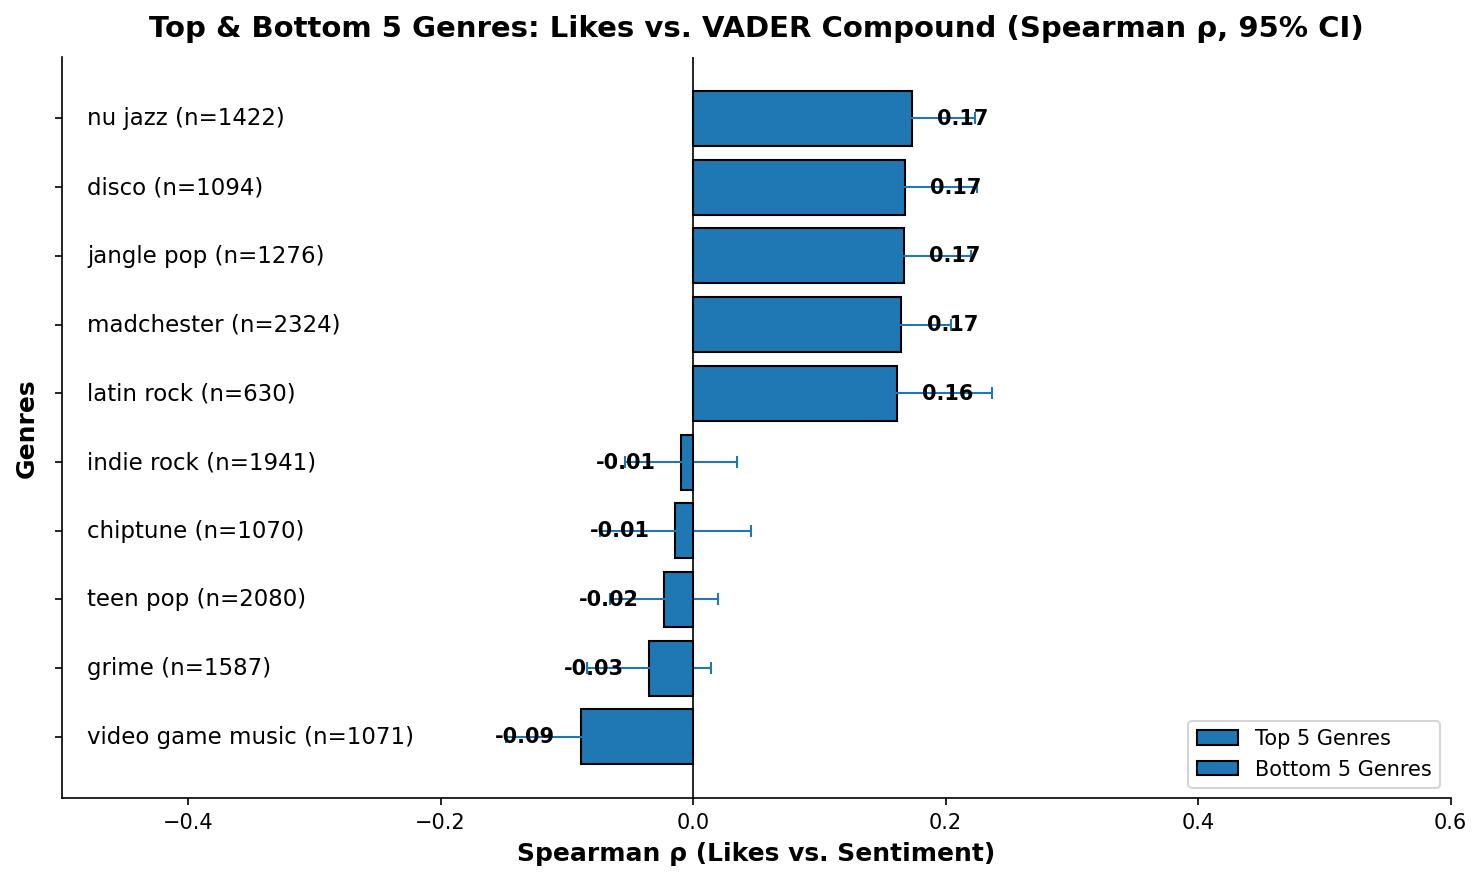
\includegraphics[width=0.85\textwidth]{images/spear_likes_comp_tb5.png}
    \caption{Top and bottom five genres by correlation between likes and VADER compound sentiment.}
    \label{fig:spear_likes_comp}
\end{figure}
\FloatBarrier

\paragraph{Summary}
Across all dimensions, correlations remain weak in absolute terms but reveal 
genre-specific endorsement norms. Positivity is rewarded in some communities 
(e.g., Nu Jazz, Disco), while others display preferences for neutrality or 
even negativity (e.g., Singer-Songwriter, Folk). These findings suggest that 
audience engagement is not uniformly driven by positive expression, but rather 
reflects culturally shaped communication patterns within each genre. As most 
comments received few or no likes, these results should be interpreted with 
caution, since the sparse engagement distribution may attenuate correlations.


\section{Sentiment Distributions Across Genres}
\label{subsec:results_distributions}

Average VADER \texttt{compound} scores across 233 genres vary substantially
(from 0.475 to 0.062; a spread of $\approx 0.41$ points on the average comment).

Spiritual and smooth genres dominate the positive end: \textit{Worship} (0.475)
is highest, followed by \textit{Smooth Jazz} (0.447), \textit{New Age} (0.433),
\textit{Gospel} (0.419), and \textit{Vocal Jazz} (0.419). Conversely, heavier and more
aggressive styles occupy the lower end: \textit{Death Metal} (0.062) and
\textit{Brutal Death Metal} (0.068), followed by \textit{Noise} (0.098),
\textit{Rap} (0.103), and \textit{Hardcore Punk} (0.104). Notably, even the lowest
averages remain above zero, implying comments are, on balance, slightly positive.
\begin{figure}[htbp]
    \centering
    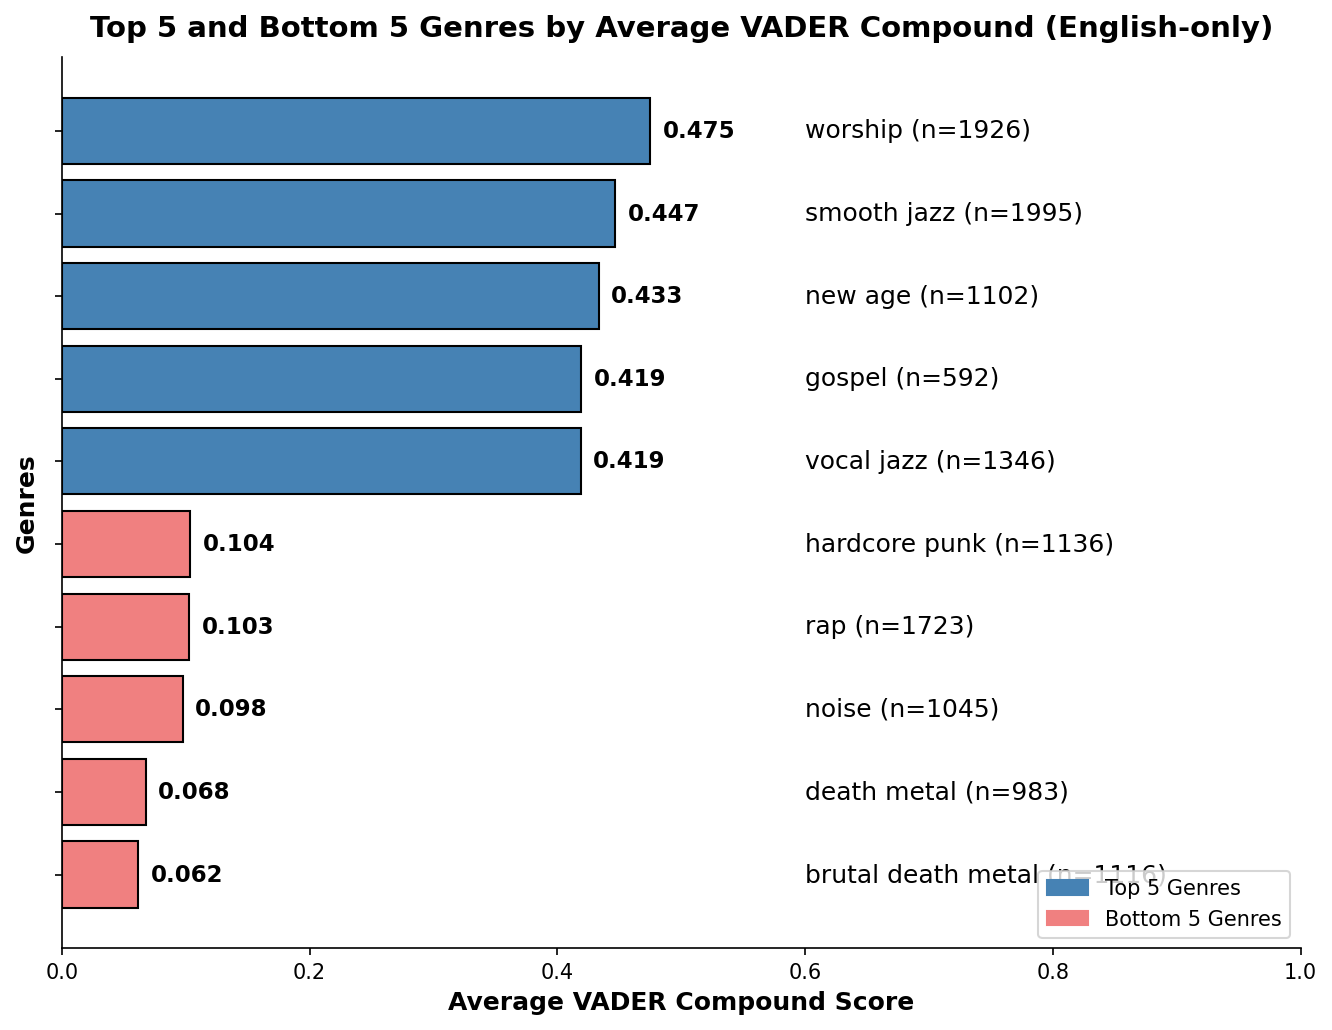
\includegraphics[width=0.8\textwidth]{images/average_vader_compound.png}
    \caption{Top 5 most positive and bottom 5 lowest-scoring genres by average compound score.}
    \label{fig:average_vader_compound}
\end{figure}
\FloatBarrier


\section{Polarity and Polarization}
\label{subsec:results_polarization}

We report \emph{within-comment} polarization using Eq.~\eqref{eq:polarity_comment}
and \emph{between-comment} polarization using Eq.~\eqref{eq:polarity_genre}.

\subsection*{Within-Comment Polarization}
\label{subsubsec:results_within}

 Extreme or intense styles (e.g., \textit{Death Metal},
\textit{Brutal Death Metal}, \textit{Technical Death Metal}) show the highest within-comment
ambivalence, indicating comments often mix strong positive and negative elements.
\textit{Spoken Word} and \textit{Doom Metal} also appear among the most polarized,
suggesting highly personal narratives or darker atmospheres elicit mixed emotions.
By contrast, genres such as \textit{World}, \textit{Cool Jazz}, and \textit{Disco}
show the lowest ambivalence, with comments tending to be one-sided.

\begin{figure}[H]
    \centering
    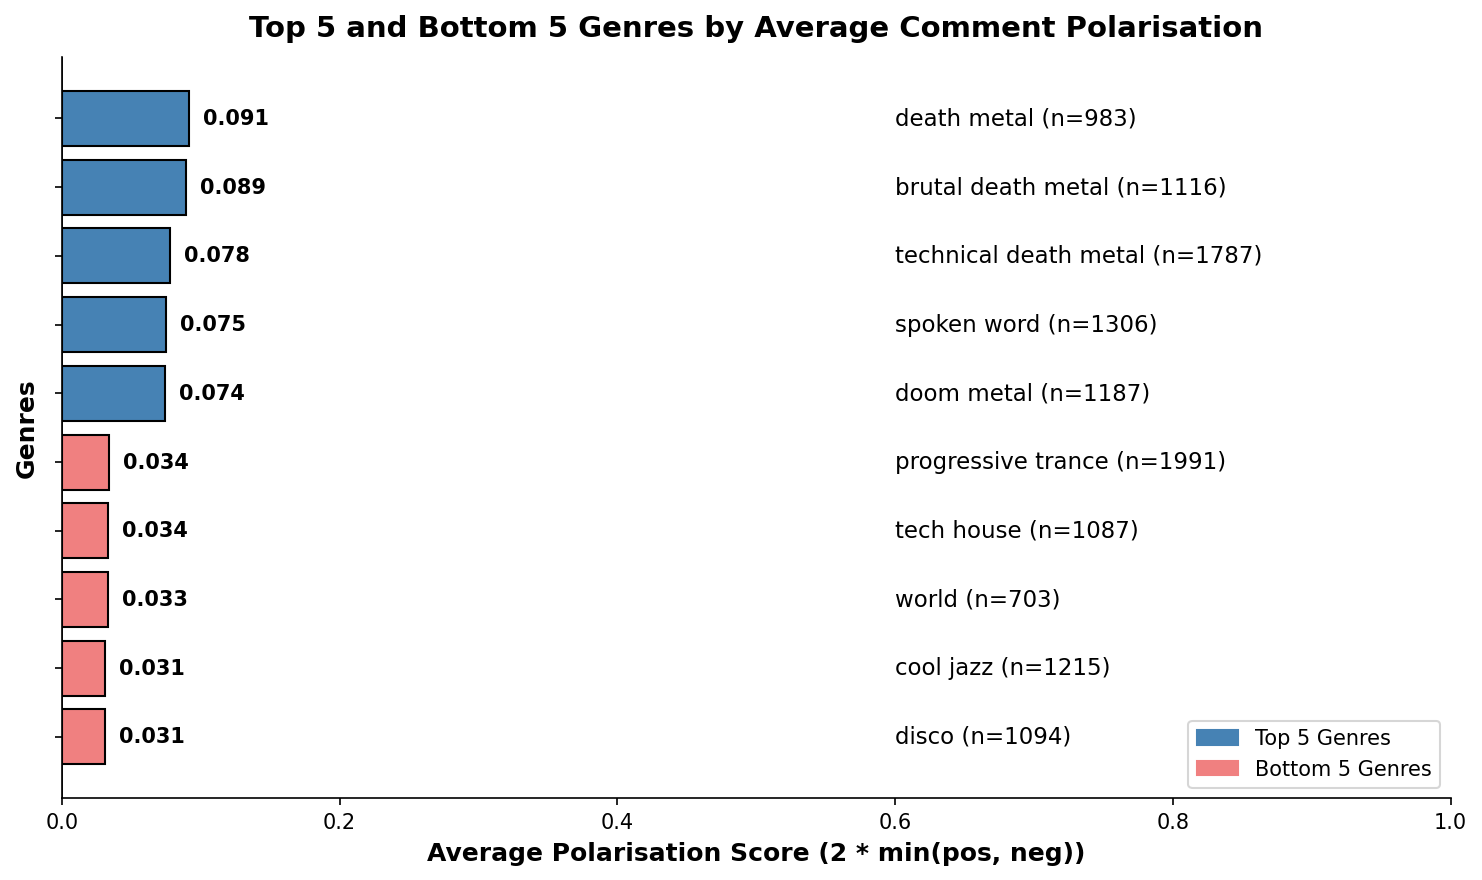
\includegraphics[width=0.85\textwidth]{images/average_polarisation.png}
    \caption{Top 5 and bottom 5 genres ranked by within-comment polarization
    ($2 \times \min(\mathrm{pos}, \mathrm{neg})$).}
    \label{fig:within_polarisation}
\end{figure}
\FloatBarrier

\subsection*{Between-Comment Polarization}
\label{subsubsec:results_between}

Aggressive styles (\textit{Brutal Death Metal}, \textit{Death Metal},
\textit{Deathcore}) are among the most polarized across comments, indicating community-level
divisiveness (strong enthusiasm coexisting with strong criticism). \textit{Noise} and
\textit{Emo Rap} also rank highly. 
By contrast, jazz-related genres as well as World and Progressive Trance show low polarization, indicating that comments there are more uniform in tone.

\begin{figure}[H]
    \centering
    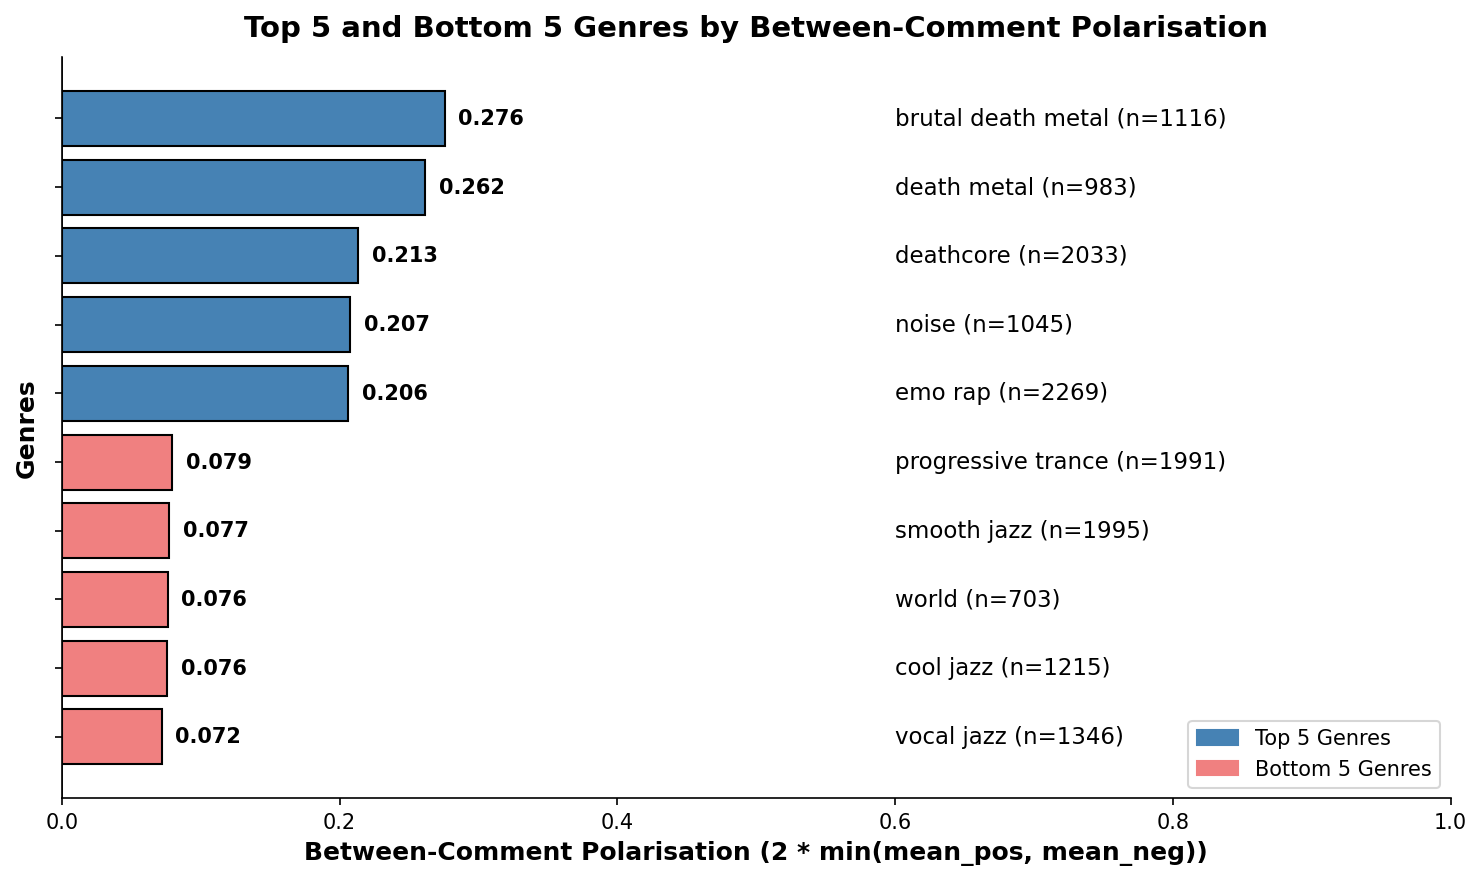
\includegraphics[width=0.85\textwidth]{images/between_polarisation_top_bottom.png}
    \caption{Top 5 and bottom 5 genres ranked by between-comment polarization
    ($2 \times \min(\overline{\mathrm{pos}}, \overline{\mathrm{neg}})$).}
    \label{fig:between_polarisation}
\end{figure}
\section{Hip-Hop Anomaly}
\label{subsec:results_hiphop}

Hip-hop genres present an unexpected pattern: despite global popularity, their compound
sentiment ranks near the bottom across genres.

\begin{table}[htbp]
\centering
\caption{Sentiment analysis for selected hip-hop genres.}
\label{tab:hiphop_sentiment}
\begin{tabular}{|l|c|c|c|c|}
\hline
\textbf{Genre} & \textbf{Positive} & \textbf{Negative} & \textbf{Neutral} & \textbf{Compound} \\
 & \textbf{Score (Rank)} & \textbf{Score (Rank)} & \textbf{Score (Rank)} & \textbf{Score (Rank)} \\
\hline
Hip Hop & 0.169 (223/233) & 0.080 (39/233) & 0.750 (18/233) & \textbf{0.173 (215/233)} \\
\hline
Alternative Hip Hop & 0.173 (217/233) & 0.085 (23/233) & 0.742 (36/233) & \textbf{0.154 (222/233)} \\
\hline
Experimental Hip Hop & 0.156 (231/233) & 0.101 (7/233) & 0.743 (33/233) & \textbf{0.124 (227/233)} \\
\hline
\end{tabular}
\end{table}

Traditional hip-hop performs best among the subgenres with an average compound of 0.173
(rank 215/233), while experimental hip-hop ranks lowest at 0.124 (rank 227/233), also
showing the 7th highest negative score overall.

\paragraph{Data Anomaly Check.}
One user contributed 66 of 5{,}418 hip-hop comments. The outlier’s mean compound was $-0.019$;
excluding the user shifts the hip-hop mean from 0.150 to 0.152 ($n=5{,}352$), a negligible change,
indicating the low scores are not driven by a single account.

\paragraph{Comparison with All Genres.}
Across 136 features, hip-hop stands out:
\emph{higher engagement} (views 16.5M vs.\ 10.5M, likes 188{,}898 vs.\ 82{,}196, comments 11{,}693 vs.\ 3{,}907)
but \emph{lower conventional positivity} (lower Tone and Positive Emotion), \emph{longer comments}
(20.7 vs.\ 17.6 words), \emph{higher emoji usage} (6.20 vs.\ 4.09), and slightly \emph{higher Authenticity}.
This combination suggests communication conventions that differ from those captured by lexicon-based sentiment.

\section{Views and Sentiment}
\label{subsec:results_views}

We correlate per-video mean compound with $\log_{10}(1+\texttt{view\_count})$.
A very weak negative correlation is observed ($r = -0.05, p < 0.001$),
indicating that more popular videos tend to have slightly lower average positivity;
however, the effect is practically negligible.

\begin{figure}[H]
    \centering
    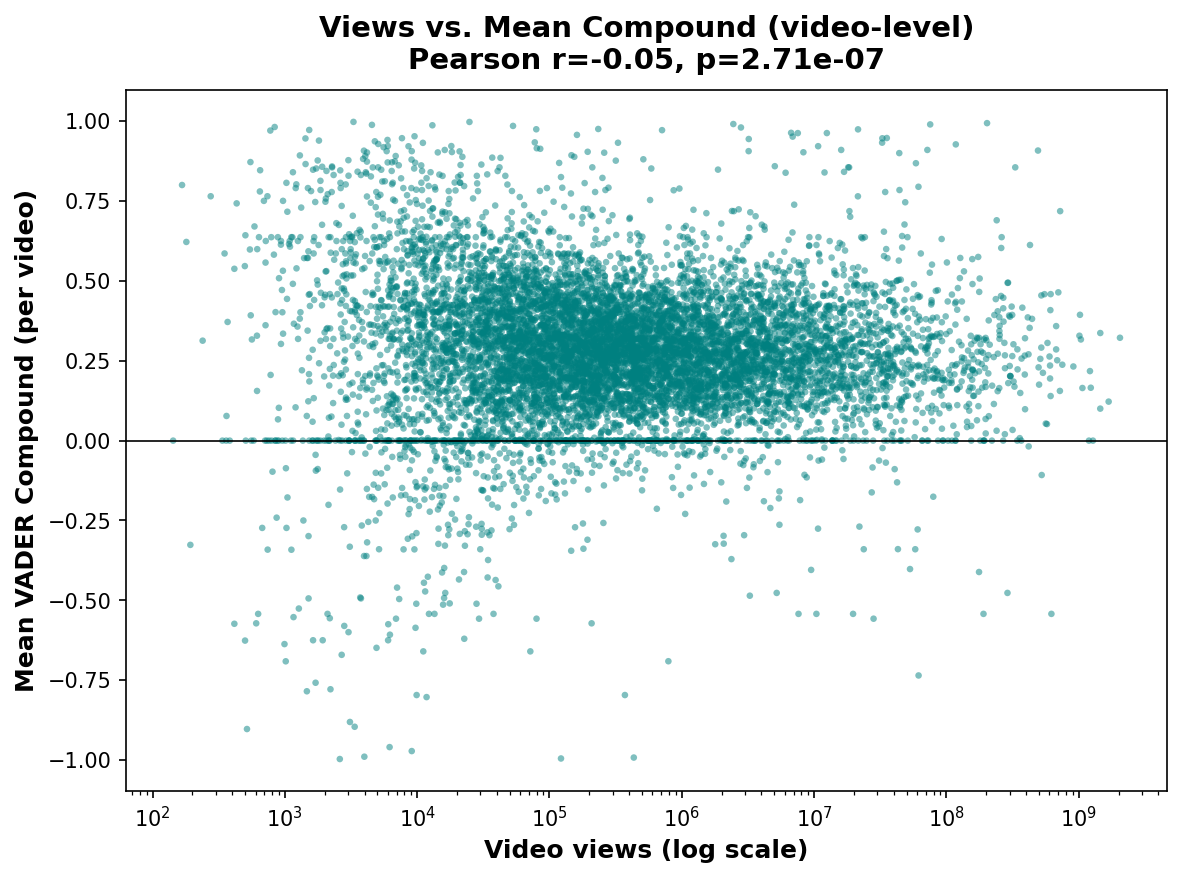
\includegraphics[width=0.85\textwidth]{images/scatter_views_vs_mean_compound.png}
    \caption{Video views (log scale) vs.\ mean VADER compound per video.
    Each point is a video; a weak negative association is visible ($r=-0.05$).}
    \label{fig:views_vs_compound}
\end{figure}

\section{Emoji Usage and Sentiment}
\label{subsec:results_emoji}

Across all comments, emoji presence is associated with higher sentiment:
average compound with emojis is \textbf{0.417} versus \textbf{0.255} without
($+64\%$ relative increase). Thus, higher emoji usage in hip-hop does not explain
its lower compound; if anything, emojis are generally linked to more positive tone.

\subsection*{Emoji Count Thresholds}
We examine thresholds $x\in\{2,3,4,5\}$ contrasting $\le x$ vs.\ $>x$ emojis:

\begin{table}[htbp]
\centering
\caption{Emoji threshold analysis: mean compound by group.}
\label{tab:emoji_thresholds}
\begin{tabular}{|c|c|c|c|c|c|}
\hline
\textbf{Threshold} & \textbf{Avg 1-to-x} & \textbf{Avg >x} & \textbf{Difference} & \textbf{n 1-to-x} & \textbf{n >x} \\
\hline
5 & 0.7896 & 0.5166 & \textbf{0.2730} & 48 & 332 \\
3 & 0.7796 & 0.5336 & 0.2460 & 27 & 353 \\
2 & 0.7897 & 0.5446 & 0.2451 & 10 & 370 \\
4 & 0.7560 & 0.5310 & 0.2250 & 34 & 346 \\
\hline
\end{tabular}
\end{table}

Comments with \textbf{1--5} emojis achieve the highest sentiment (0.7896),
whereas $>5$ emojis corresponds to lower scores (0.5166). Hip-hop’s mean of 6.20
places many comments beyond this optimal range.

Moderate emoji usage aligns with the highest median
compound and smaller spread. No-emoji comments show lower medians and wider spread;
$>5$ emojis are still positively biased but less consistently so.


\begin{figure}[H]
    \centering
    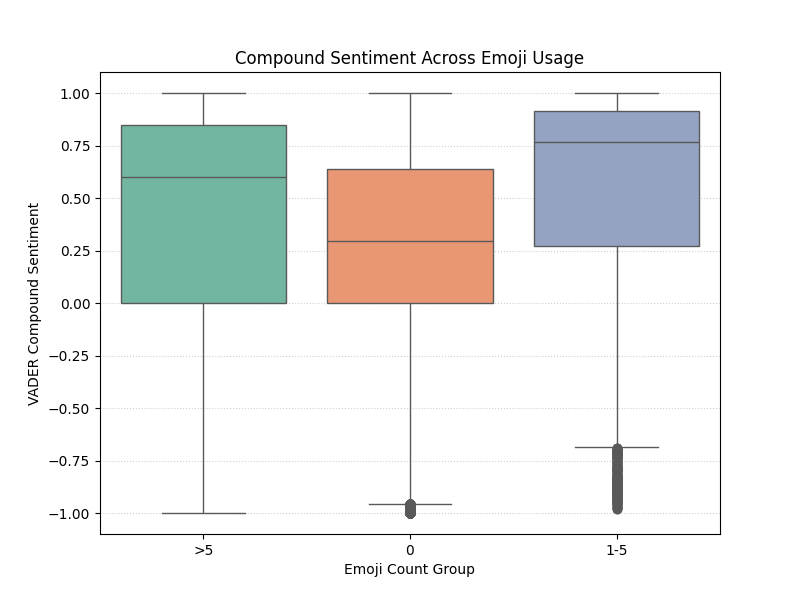
\includegraphics[width=0.75\textwidth]{images/boxplot_emoji_compound.png}
    \caption{Distribution of compound scores across three emoji groups:
    no emojis, 1--5 emojis, and $>5$ emojis.}
    \label{fig:emoji_boxplot}
\end{figure}
\FloatBarrier


\section{LIWC Dimensions and Cultural Markers}
\label{subsec:results_liwc}

We compare genres on LIWC features to contextualize stylistic and cultural
differences beyond sentiment.

\paragraph{Positive vs.\ Negative Balance.}
The balance index $(\texttt{emo\_pos} - \texttt{emo\_neg})$ ranks spiritual and jazz genres
highest, with hip-hop among the lowest, reinforcing lexicon-based lower positivity.

\begin{figure}[htbp]
    \centering
    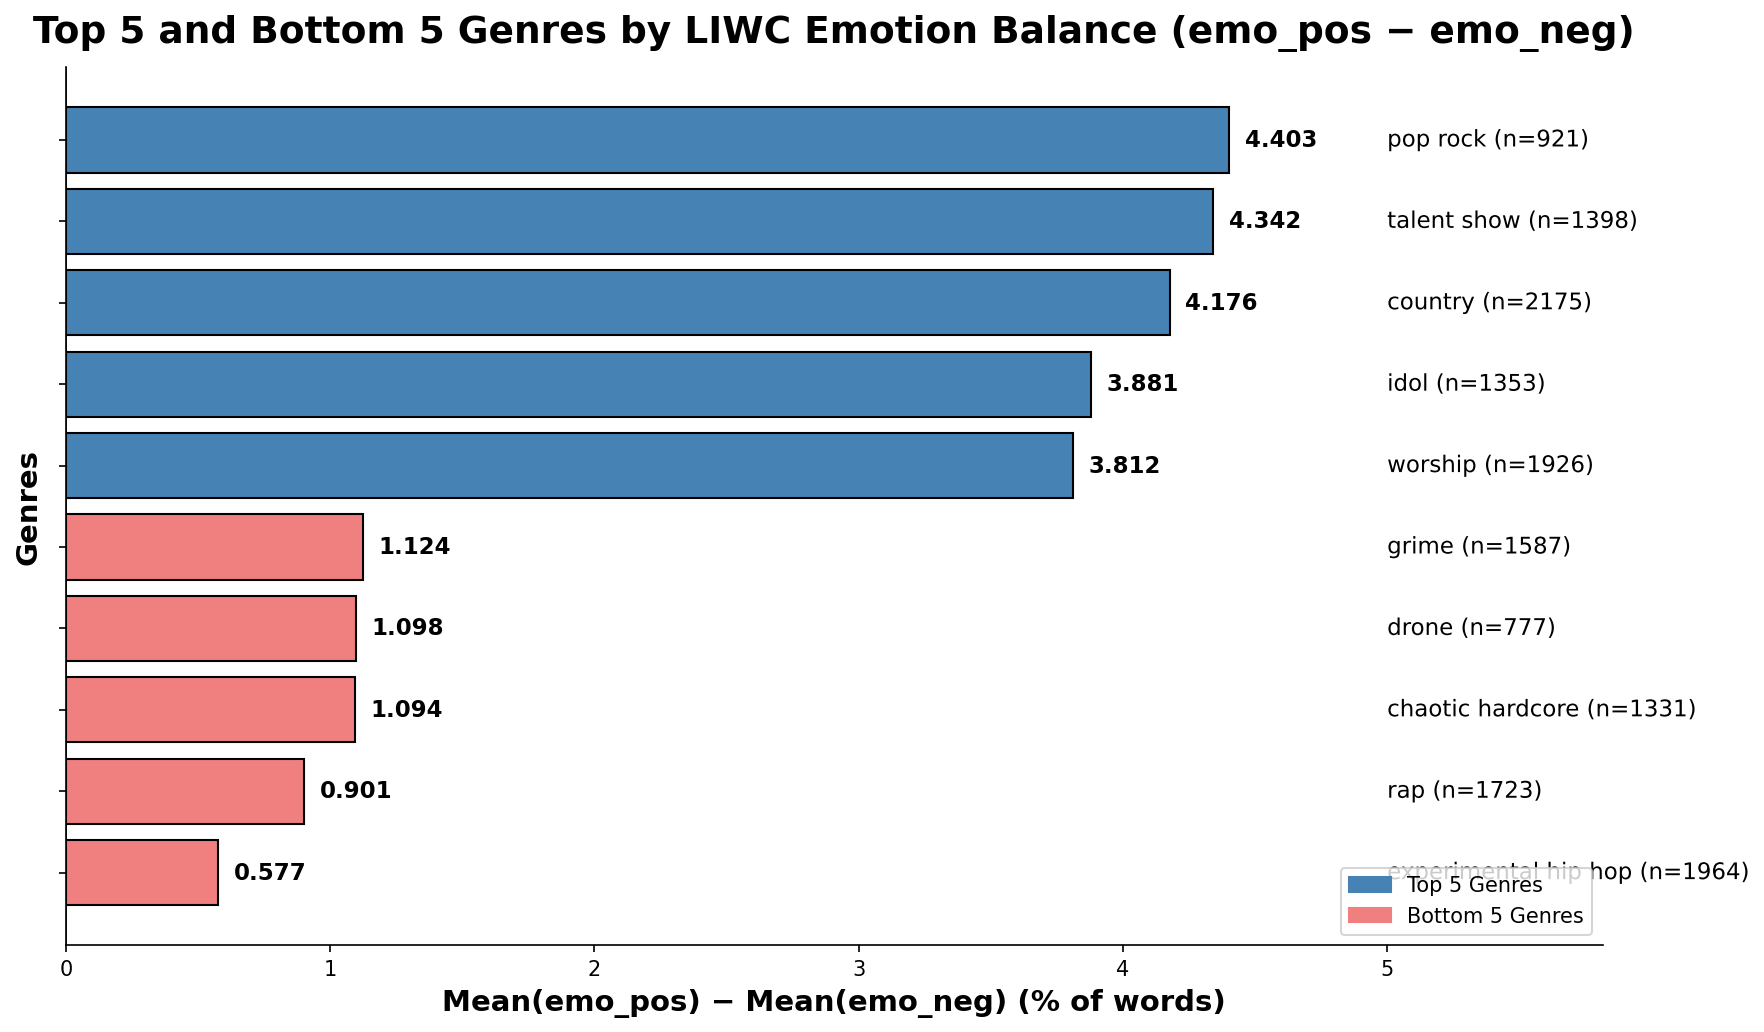
\includegraphics[width=0.7\linewidth]{images/top_bottom_emopos_emoneg.png}
    \caption{Top and bottom genres by LIWC \texttt{emo\_pos} minus \texttt{emo\_neg} balance.}
    \label{fig:liwc_emopos_emoneg_balance}
\end{figure}

\paragraph{Swear, Conflict, and Social.}


The \texttt{Swear} category captures the frequency of swear and offensive words, while 
\texttt{Conflict} refers to words denoting disagreement. Both are highest in 
aggressive metal genres and lowest in worship and gospel 
(Figures~\ref{fig:liwc_swear} and~\ref{fig:liwc_conflict}). 
In contrast, the \texttt{Social} category measures words related to social relations 
(e.g., friend, talk, share). This language is most frequent in \textit{Worship}, 
\textit{Country Pop}, and \textit{K-pop}, and least common in extreme metal subgenres 
(Figure~\ref{fig:liwc_social}).

\begin{figure}[htbp]
    \centering
    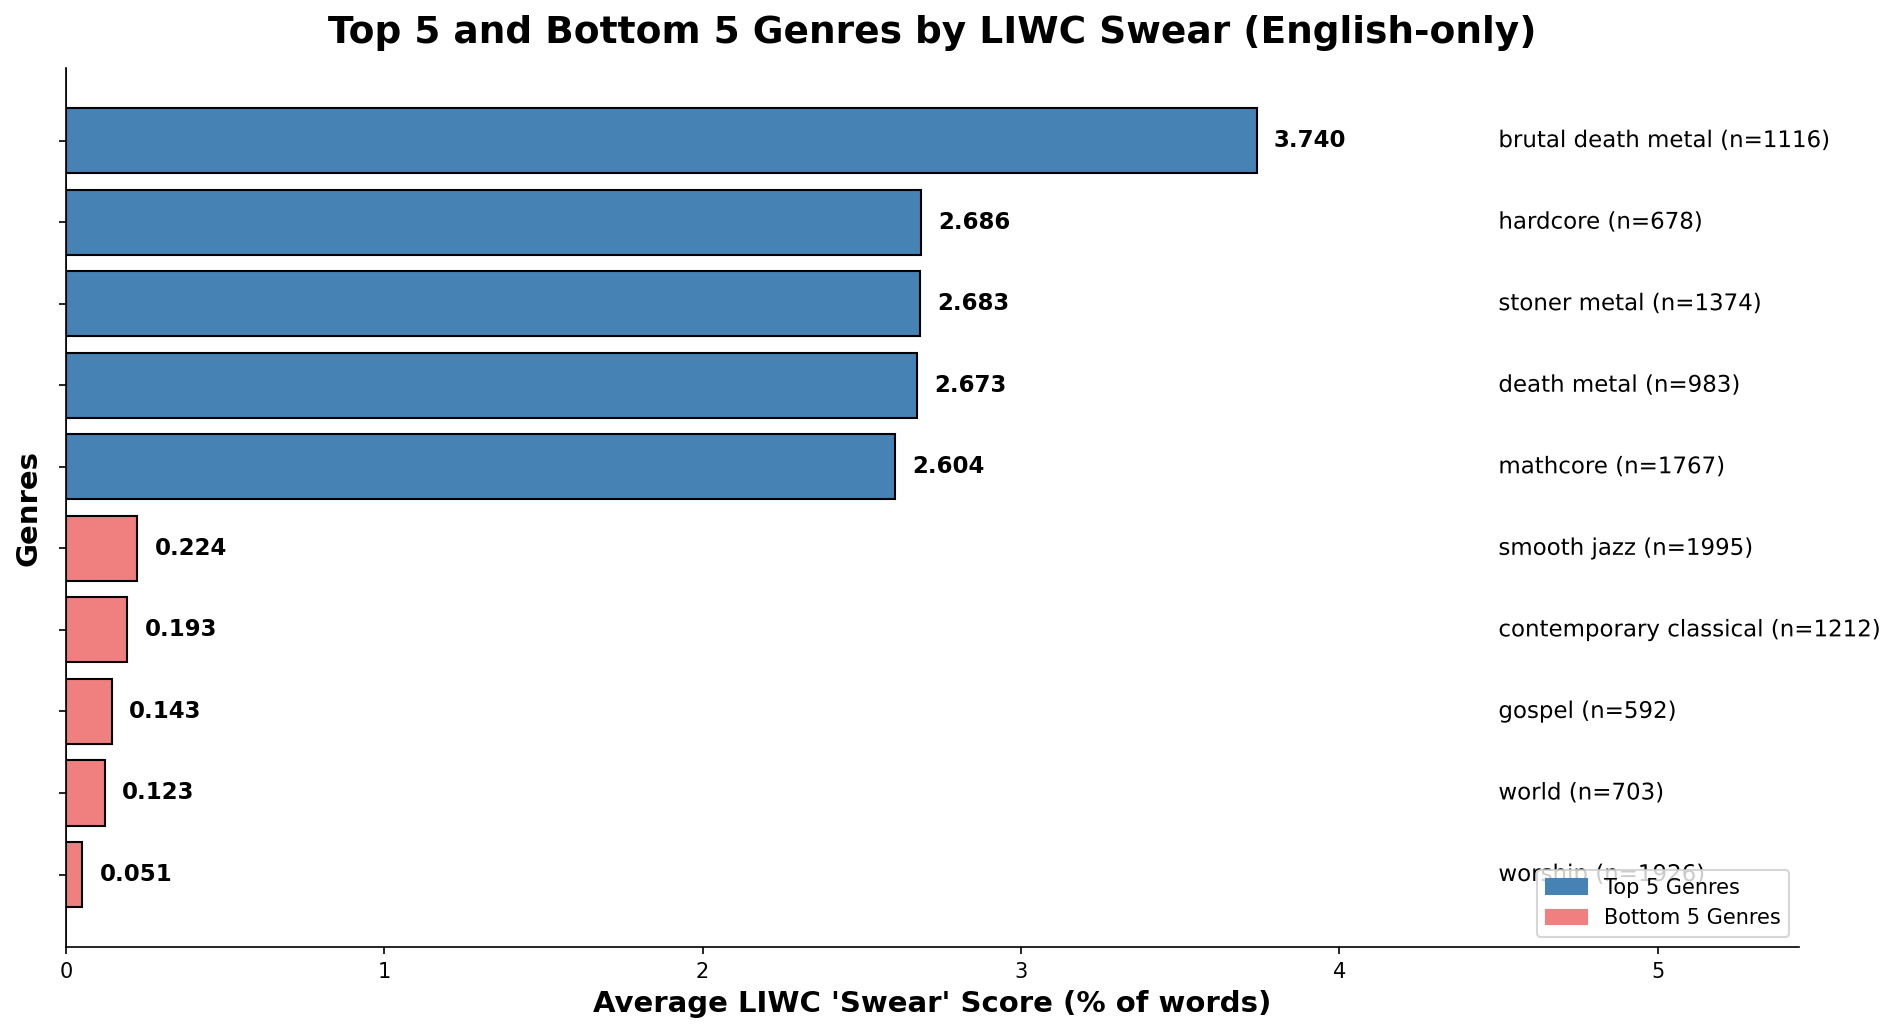
\includegraphics[width=0.8\linewidth]{images/swear.png}
    \caption{Top and bottom genres by LIWC \texttt{Swear}.}
    \label{fig:liwc_swear}
\end{figure}

\begin{figure}[htbp]
    \centering
    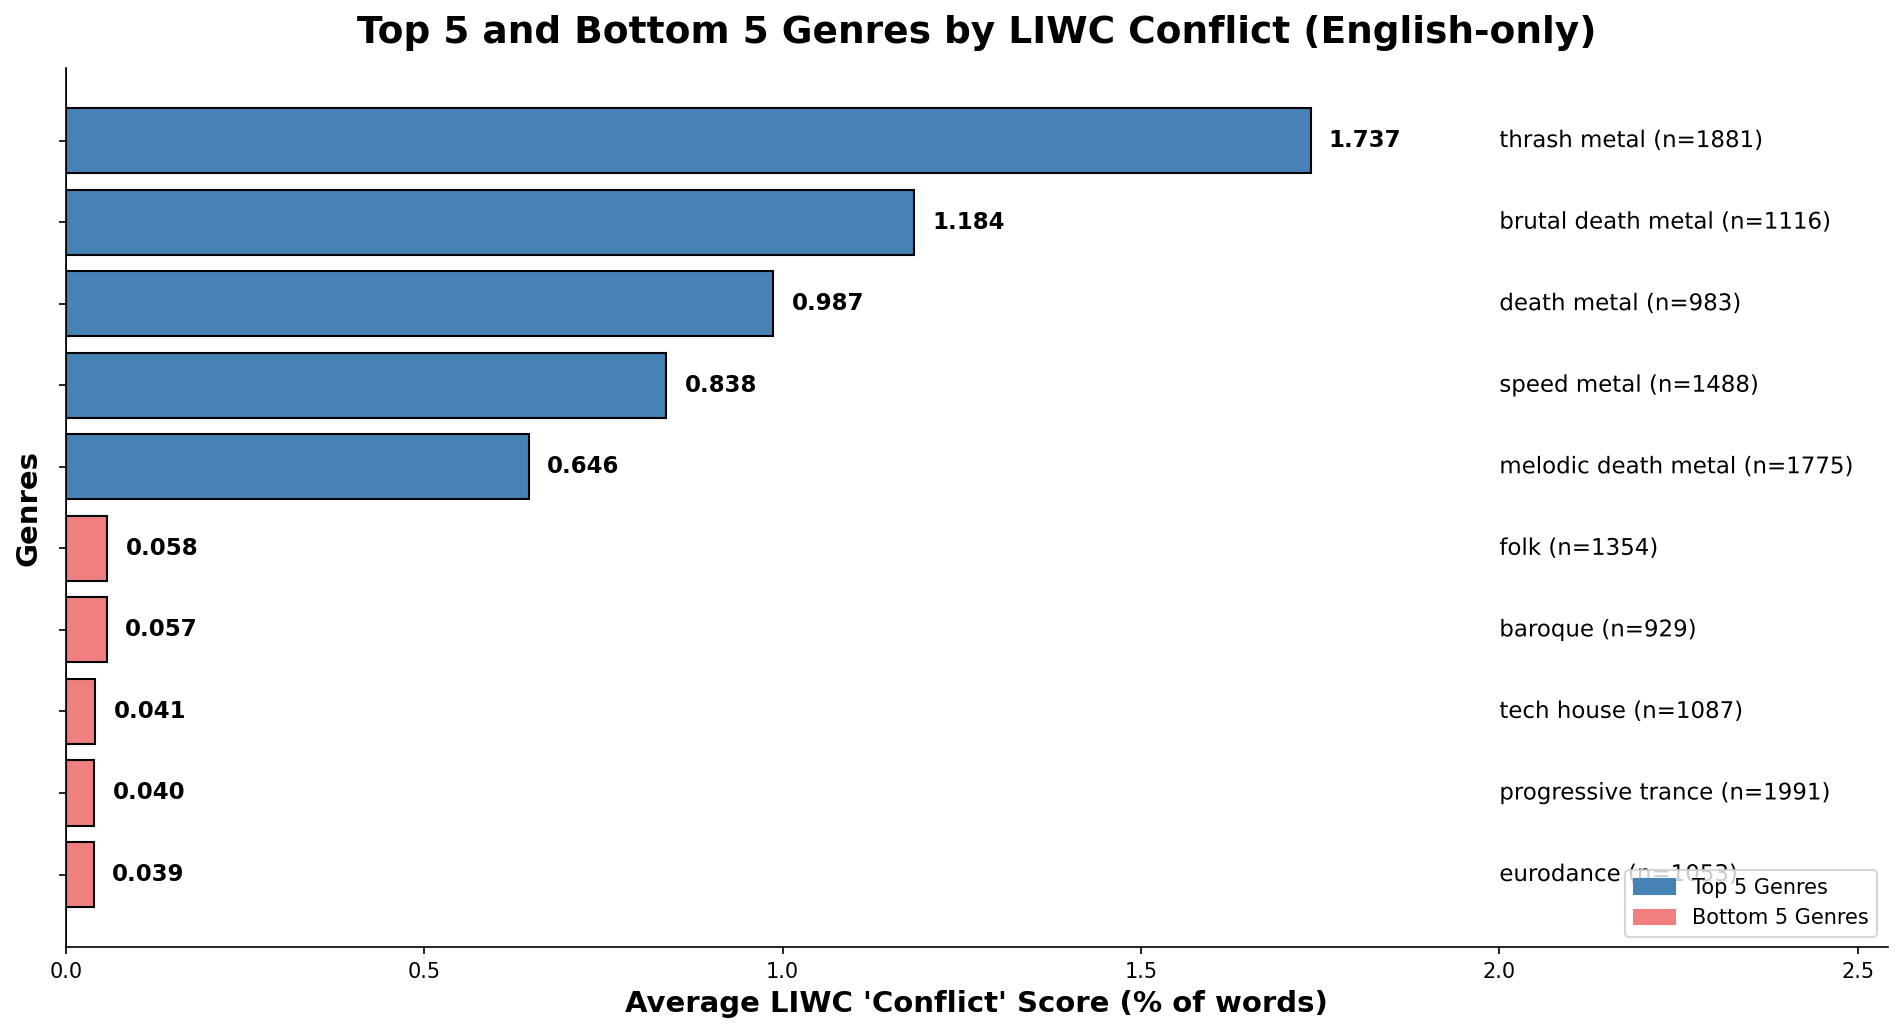
\includegraphics[width=0.8\linewidth]{images/conflict.png}
    \caption{Top and bottom genres by LIWC \texttt{Conflict}.}
    \label{fig:liwc_conflict}
\end{figure}

\begin{figure}[htbp]
    \centering
    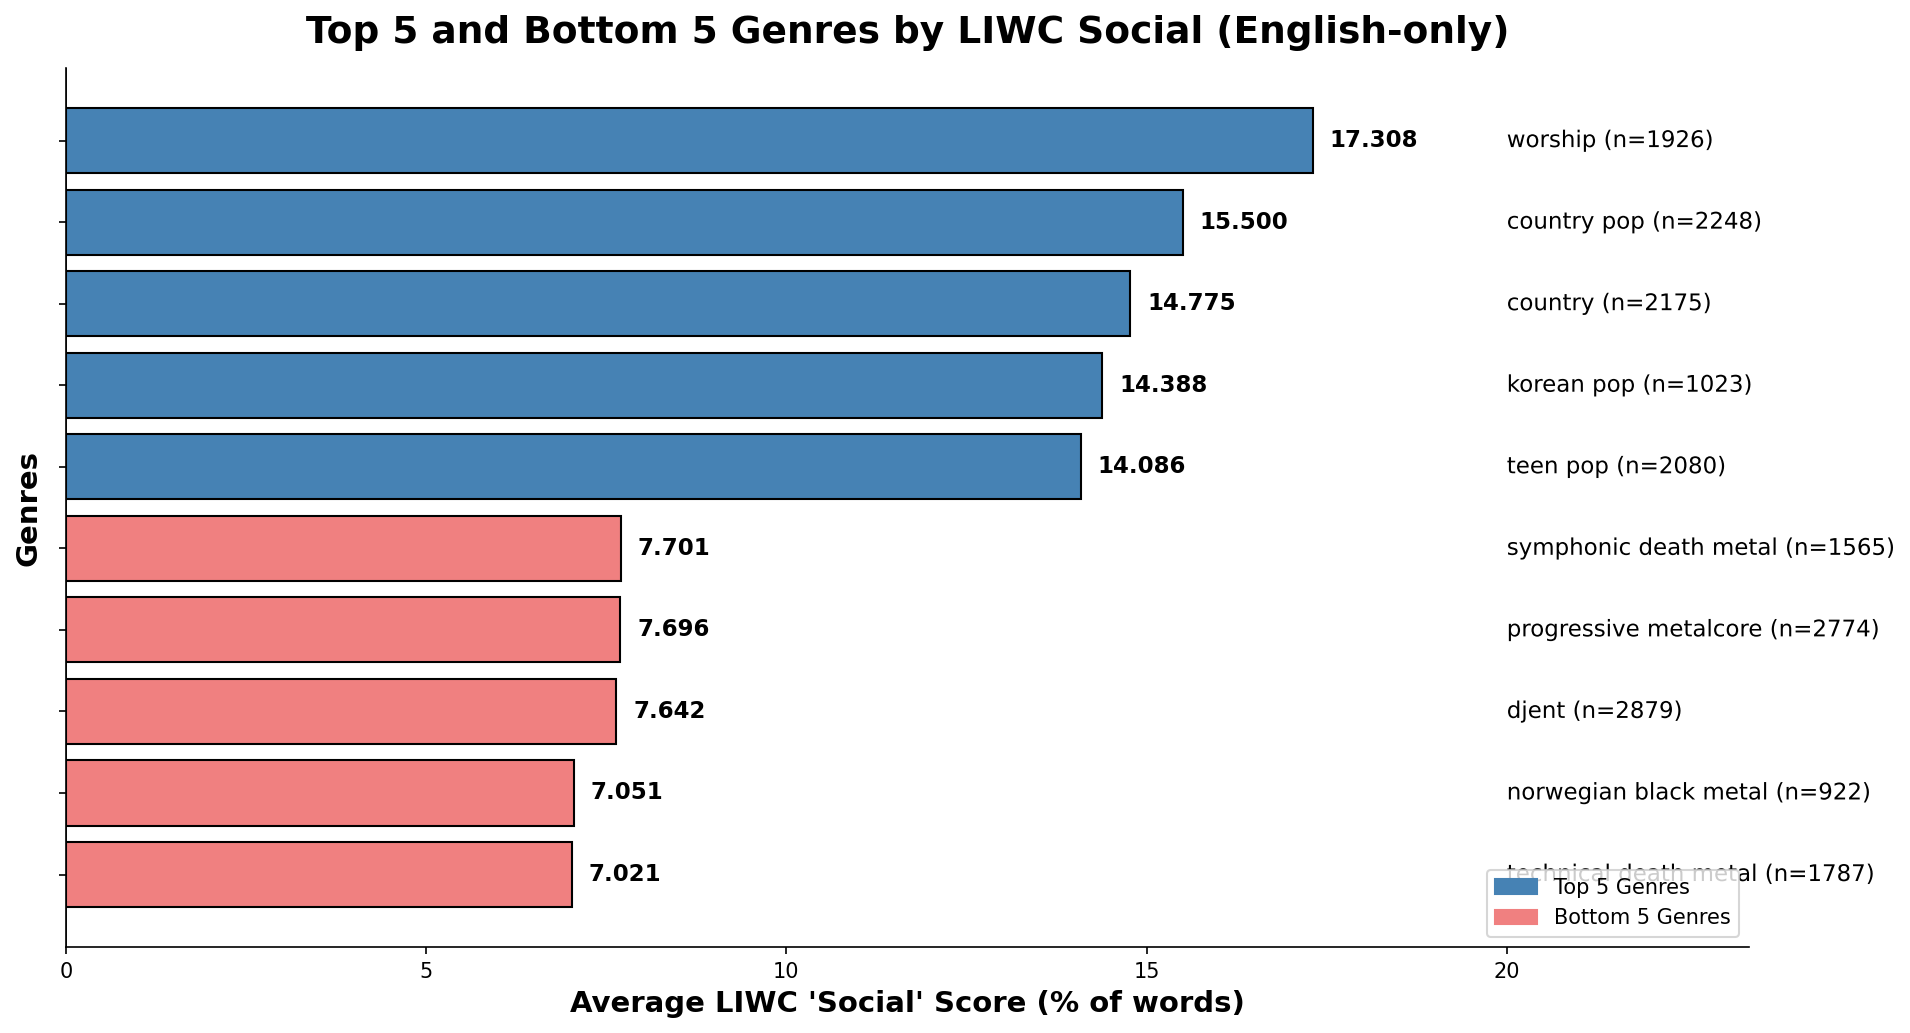
\includegraphics[width=0.8\linewidth]{images/social.png}
    \caption{Top and bottom genres by LIWC \texttt{Social}.}
    \label{fig:liwc_social}
\end{figure}

\section{LIWC--VADER Correlations}
\label{subsec:results_liwc_vader}

We correlate all LIWC dimensions with VADER sentiment (\texttt{positive}, \texttt{negative},
\texttt{neutral}, \texttt{compound}).

\begin{figure}[H]
    \centering
    \includegraphics[width=0.9\textwidth]{images/liwc_vader_correlation_filtered.png}
    \caption{Correlation of LIWC features with VADER sentiment across all comments.
    Red = positive correlation; blue = negative.}
    \label{fig:liwc_vader_corr}
\end{figure}

\paragraph{Expected patterns.}
\textit{Affect}/\textit{Emotion}/\textit{Positive Tone} correlate strongly with VADER positive
($r \approx 0.43$--$0.66$); \textit{Negative Tone}/\textit{Negative Emotion} correlate with
VADER negative ($r \approx 0.36$--$0.49$). \texttt{Swear} is positively associated with
VADER negative ($r \approx 0.37$). Neutral scores inversely track affective LIWC categories.

\paragraph{Unexpected patterns.}
The Emotion category (words directly expressing feelings such as happy, love, sad, or angry) shows a much stronger correlation with positive VADER scores than with negative ones. This is unexpected because one might assume emotional words would align equally with both valences, yet the results suggest that positive emotional language dominates in driving sentiment scores. A possible reason is that most comments are positively skewed, which could explain the stronger positive tendency.

%%%%%%%%%%%%%%%%%%%%%%%%%%%%%%%%%%%%%%%%%%%%%%%%%%%%%%%%%%%%%%%%%%%%%%%%%%%%%%%%
